\documentclass[12pt]{article}
\usepackage[utf8]{inputenc}
\usepackage{fullpage}
\usepackage{color}
\usepackage{listings}
\usepackage{graphicx}
\title{CSC 431 Compiler Report}
\date{}
\author{Austin Wise, Ryan Schroeder}

\begin{document}
\maketitle
\tableofcontents

\pagebreak

\section{Architecture}

A small data flow engine hooks all the pieces of the compiler together.
First we parse the command line arguments.
Based on the values we obtain from the argument parser we construct a tree of tasks that represents the actions we are going to perform.
The nodes in the tree represent the actions, the edges pass data from one node to its dependants.
Next, using our Step.DoAll function we execute each step in a topological sorted order.

\begin{figure}
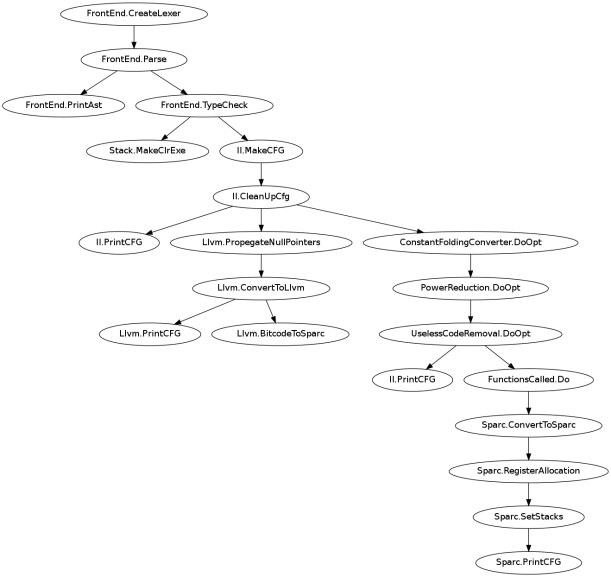
\includegraphics{compSteps.png}
\caption{Handling the two exceptions.}
\label{success}
\end{figure}

	
\pagebreak

\section{Representation of Key Data}


\subsection{Instructions}
base instruction class has source and destination sources to assist with optimizations and register allocation
for each instruction type we use a T4 template to generate specific subclasses for each individual instruction
these templates also generate a miloc converter and imiloc translator to aid in translating miloc to sparc

\subsection{Control Flow Graph}
base node class represents abstract node
specific nodes for if/loop/basic blocks/series of nodes
all nodes have a generic type parameter to ensure that they only hold instructions of one type, e.g. sparc/miloc

\section{Optimizations Implemented}
\section{Performance of the Benchmarks}
  
\end{document}
